\subsection{COCO: Die dritte Generation}

\begin{frame}
	{CommonCrawl}
	\begin{itemize}
	  \item sehr große Mengen von Crawldaten frei verfügbar
	  \item Sitz in USA, gedeckt durch Fair Use
	  \item archiviert unter Amazon Public Datasets-Programm
	  \item TB-weise über HTTP runterladbar (alternativ S3)
	\end{itemize}
\end{frame}


\begin{frame}
	{COCO: Common COW}
	\begin{itemize}
	  \item Daten-Derivate sind rechtlich unproblematisch
	  \item unsere eigentlich Leistung: \alert{Derivate}, also die Bereinigungen, Qualitätsmaße und Annotationen
	  \item Idee: \alert{Derivate von uns frei (CC-BY),\\Primärdaten von CommonCrawl}

	  \vspace{0.5cm}

	  \item Nebeneffekt: Massencrawling ist ein mühsames und\\gefährliches Unterfangen, wird dadurch gespart
	\end{itemize}
\end{frame}


\begin{frame}
	{COCO Arbeitsablauf}
	\centerinag
	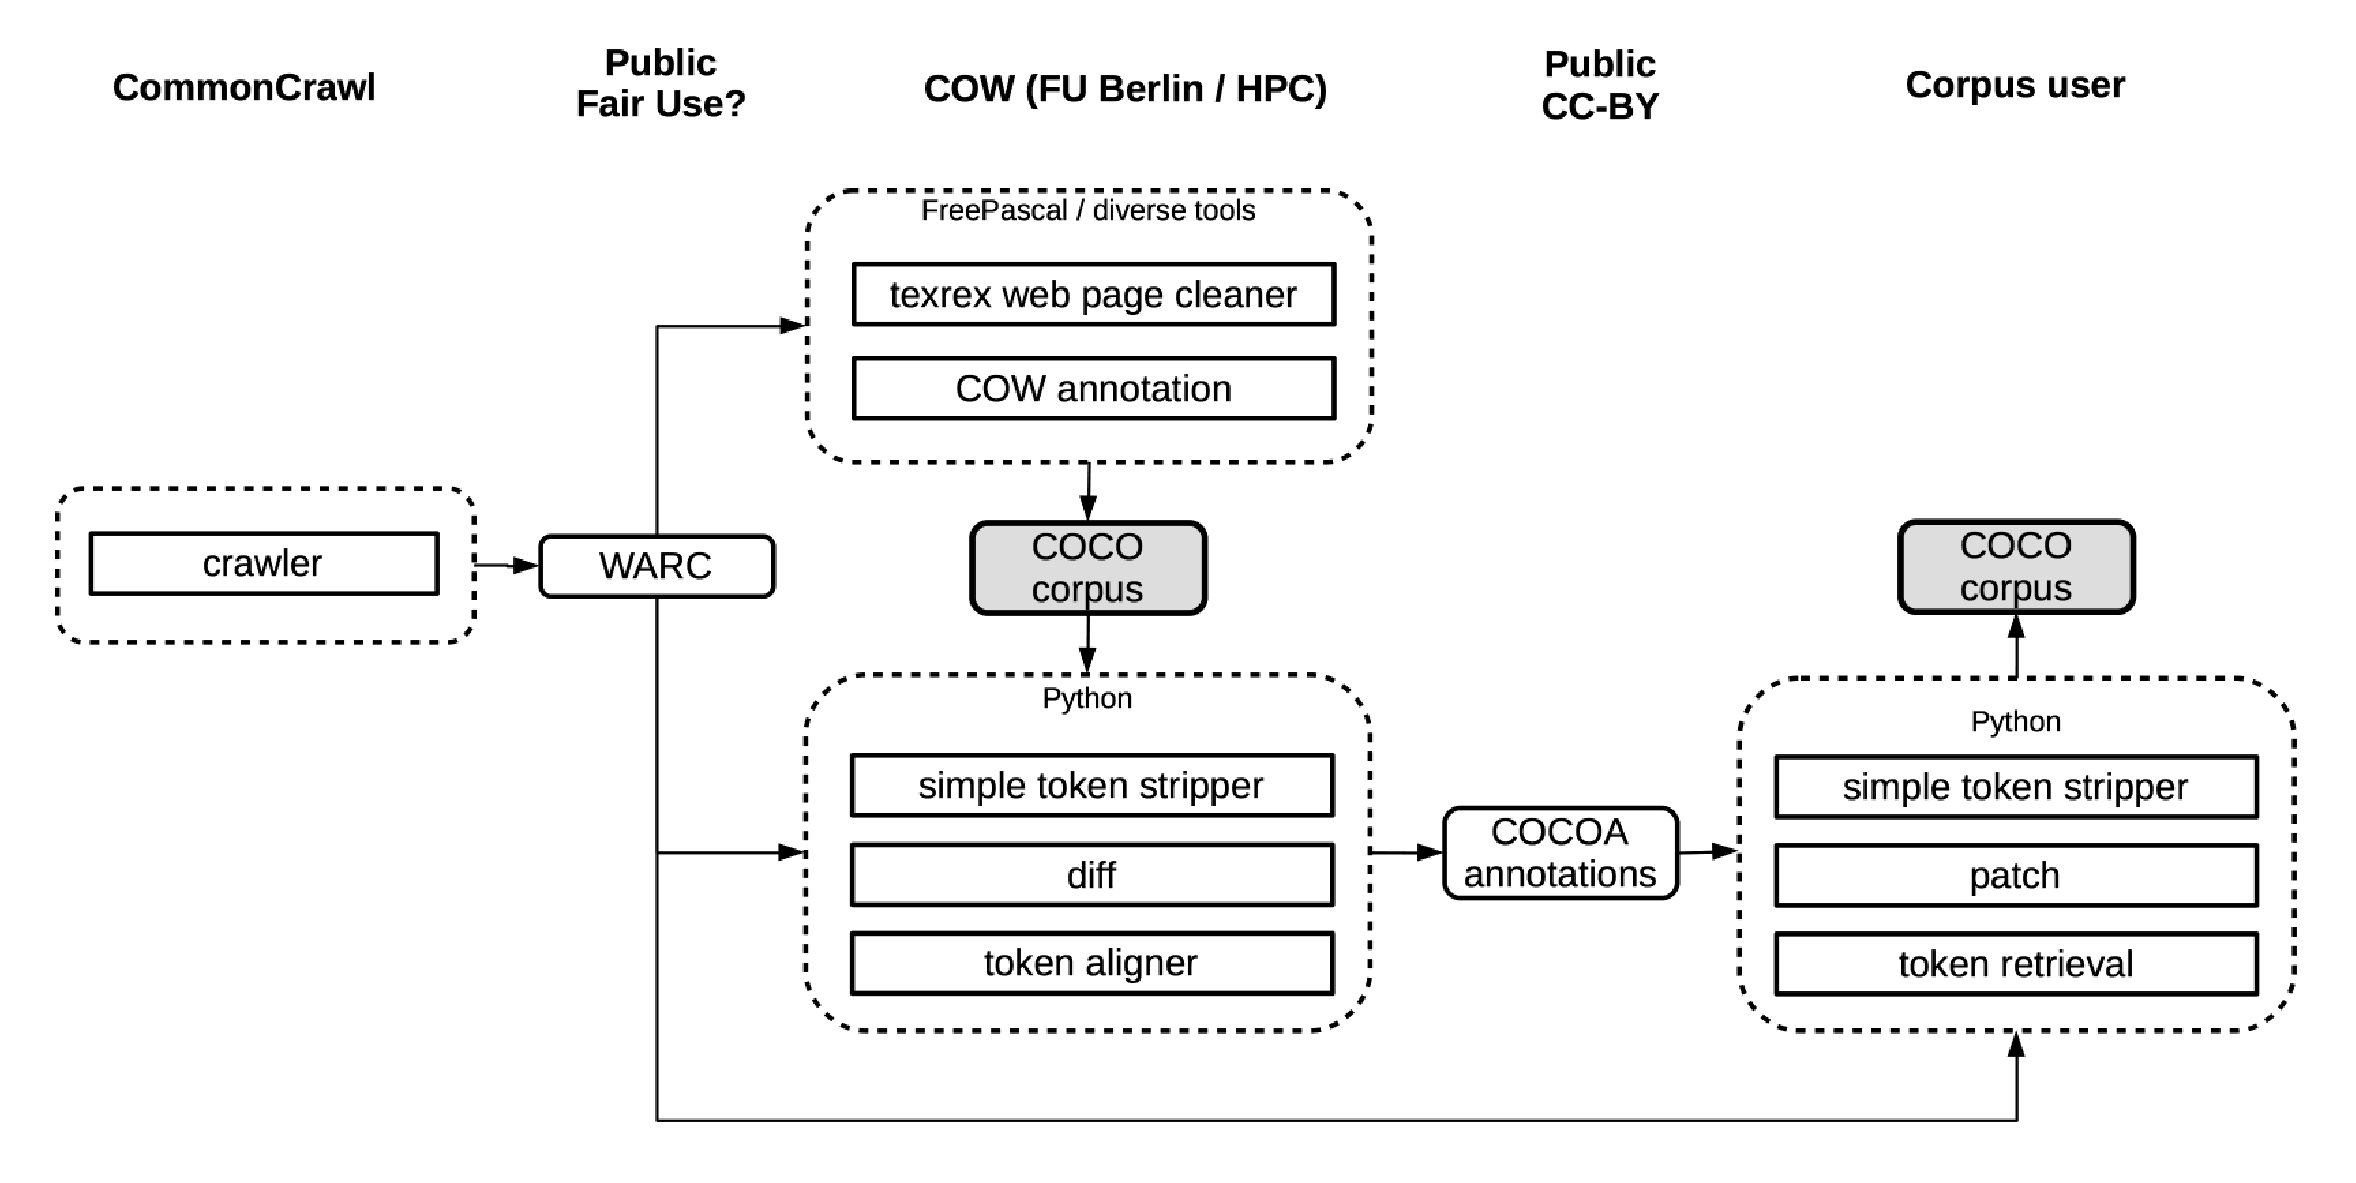
\includegraphics[width=0.9\textwidth]{graphics/workflow}
\end{frame}


\begin{frame}
	{Beispiel für COCOA-Datenformat}

	\centering
	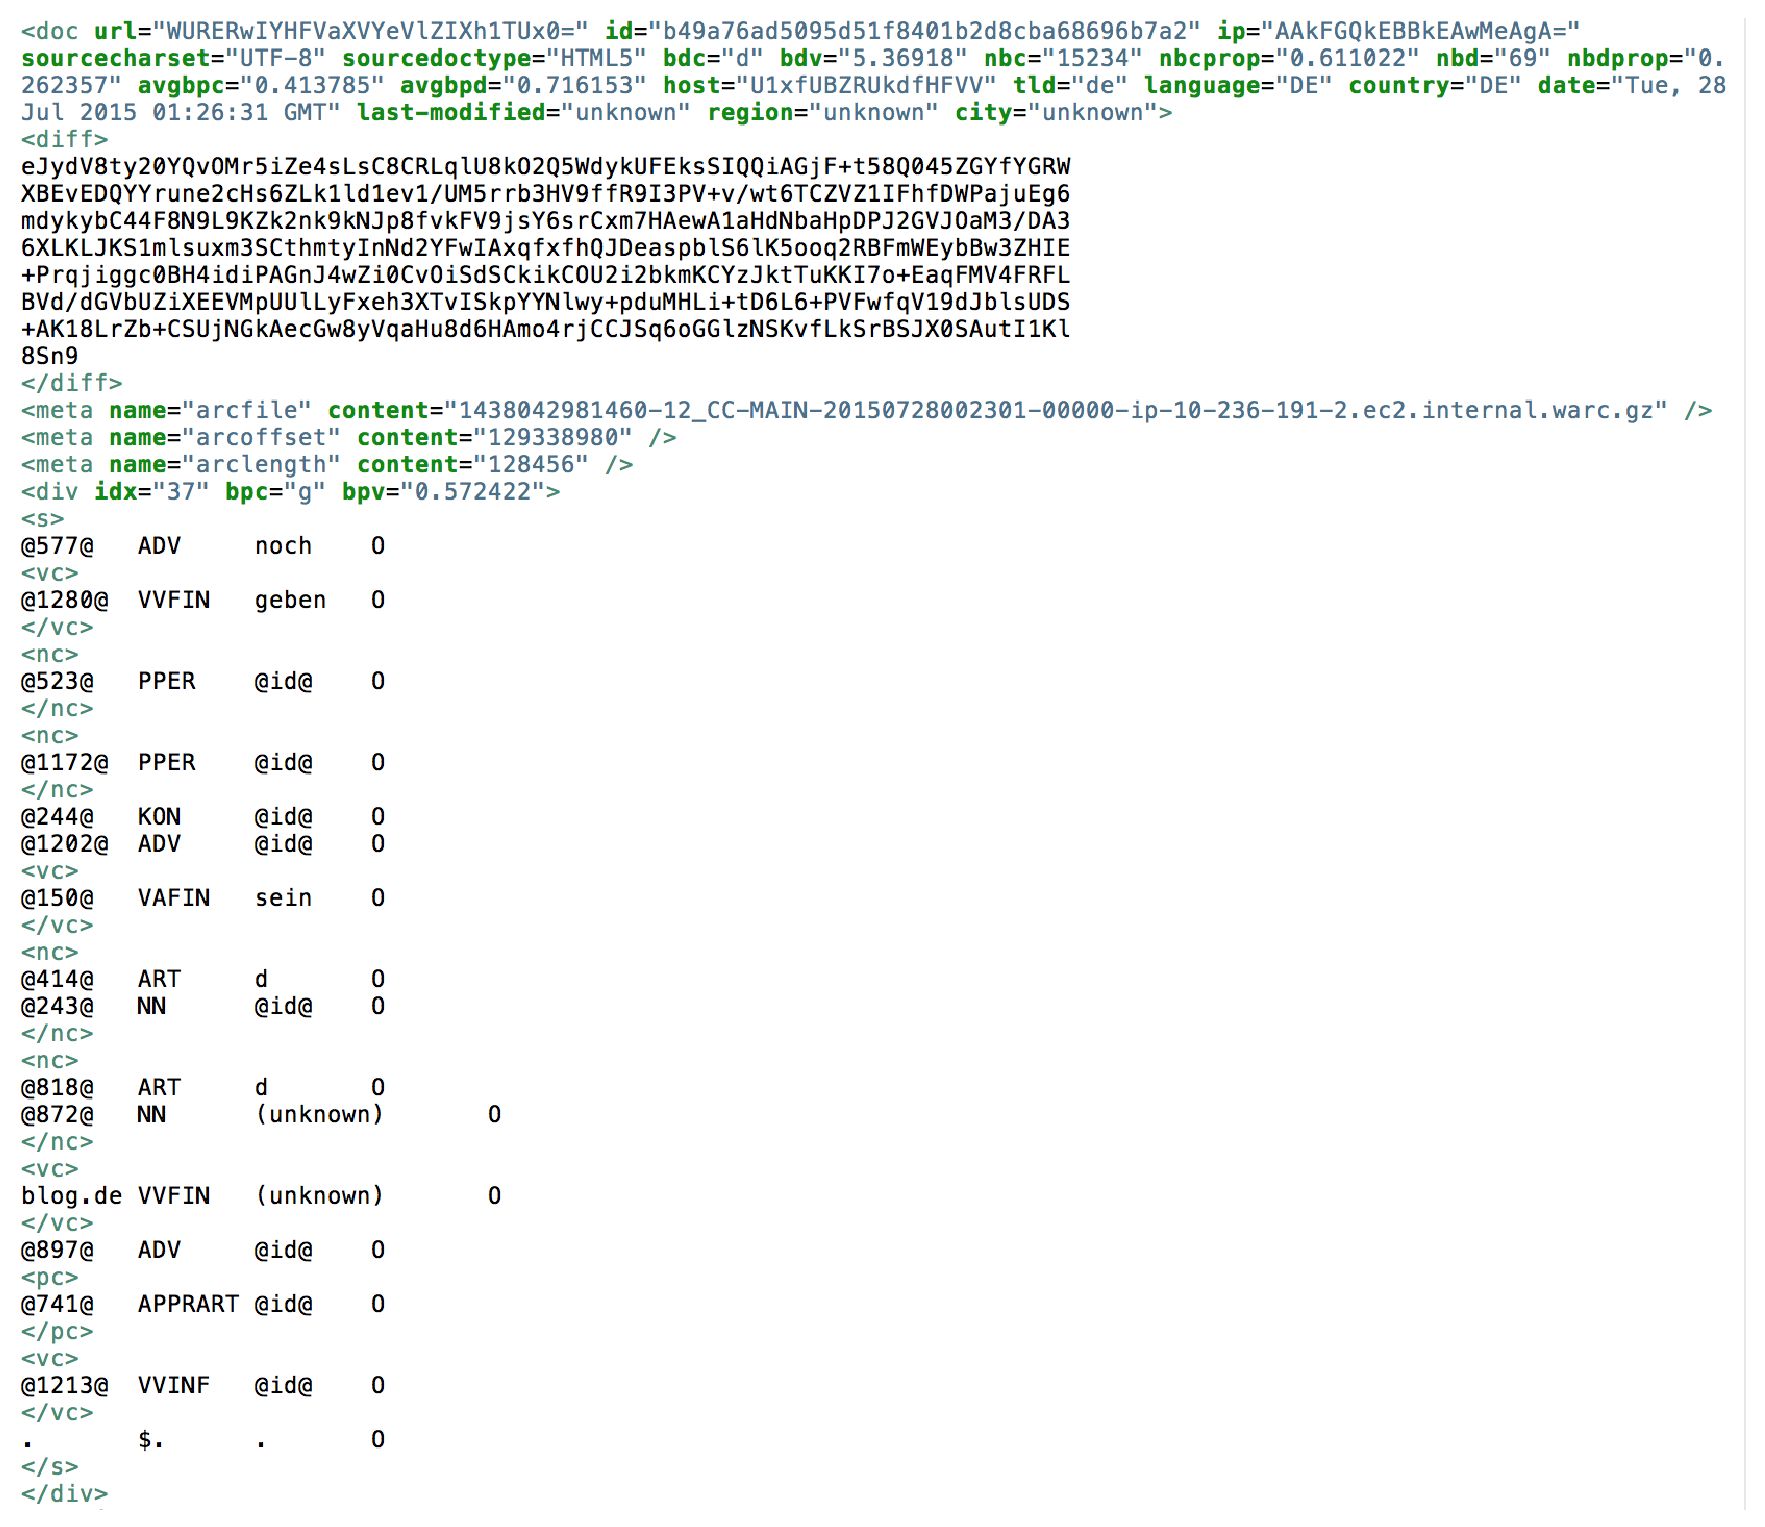
\includegraphics[height=0.85\textheight]{graphics/cocoa}
%	\scalebox{0.4}{\ttfamily
%	\begin{tabular}{llllll}
%		\hline
%		\multicolumn{6}{l}{<doc url="6ad87fe6a1b26920e1fd27eaf334" offset="92575231" length="12331">} \\
%		<s> &&&&& \\
%		<vc> &&&&& \\
%		@8702@5@  & VB   &   check  & 1  &    0    &   null \\
%		</vc> &&&&& \\
%		<nc> &&&&& \\
%		@8708@3@  &   DT    &  <id />   &  2  &     6  &     det \\
%		@8712@2@    &  NP     & <id />   &   3    &   6   &    poss \\
%		\&apos;s & POS  &   \&apos;s &4    &   3  &     possessive \\
%		</nc> &&&&& \\
%		<nc> &&&&& \\
%		@8718@7@ &NP   &   <id /> &5  &     6   &    nn \\
%		@8726@7@ &NN  &    <id /> &6      & 1   &    dobj \\
%		</nc> &&&&& \\
%		<advc> &&&&& \\
%		@8734@12@ &   RB   &   <id /> &   7   &    1    &   advmod \\
%		</advc> &&&&& \\
%		<pc> &&&&& \\
%		@8747@3@ &    IN    &  <id />  &   8   &    1   &    prep \\
%		<nc> &&&&& \\
%		@8751@7@ &NNS   &  update & 9   &    8     &  pobj \\
%		</nc> &&&&& \\
%		</pc> &&&&& \\
%		.     &  SENT  &  .   &    10  &    1   &    punct \\
%		</s> &&&&& \\
%		\hline
%	\end{tabular}}	
\end{frame}

